\section{Tips \& Tricks}

\subsection{Daha Hızlı KMeans}
\begin{lstlisting}[language=Python]
# Slow
clf = KMeans(n_clusters=7).fit(X)

# Fast
from sklearn.random_projection import SparseRandomProjection
srp = SparseRandomProjection(n_components=6)
X_srp = srp(X)
clf = KMeans(n_clusters=7).fit(X_srp)
\end{lstlisting}

\subsection{join vs iteration}
Join fonksiyonu iterasyonla eklemeden (sentence += word) daha hızlı çalışır.

\subsection{Activation Function Layer vs Parameter}
Aktivasyon fonksiyonunu katman olarak eklemek parametre olarak eklemekten daha hızlı çalışır.

\subsection{Matplotlib - Subplot Mosaic}
subplots() fonksiyonu eşit boyutlarda grafikler oluştururken, subplot\_mosaic() fonksiyonu farklı ölçeklerde grafikleri tek bir figürde göstermeyi sağlar.

\begin{lstlisting}[language=Python]
ax = fig.subplot_mosaic("""AAB
                           CCC
                           DEF""")

ax["A"].plot()
ax["B"].scatter()
ax["C"].bar()
ax["D"].pie()
ax["E].bar()
ax["F"].plot()
\end{lstlisting}

\subsection{Dont use time.time()}
Model süresini hesaplarken time.time() kullanma. Time.time() güncel zamanı hesaplar. Bunun yerine time.perf\_counter() kullan.

\subsection{DeOldify - Video/Resim Renklendirme}
Siyah-beyaz görüntü/videoları renkli hale getirmek için kullanılan önceden eğitilmiş bir modeldir. Modeli websitesinden indirip proje içerisindeki models klasörüne koymak gerekiyor.

\subsubsection{Resim Renklendirme}
\begin{lstlisting}[language=Python]
from deoldify import device
from deoldify.device_id import DeviceId
from deoldify.visualize import get_image_colorizer, show_image_in_notebook
import warnings
warnings.filterwarnings("ignore")
device.set(device=DeviceId.GPU0)

colorizer = get_image_colorizer(artistic=True)
render_factor = 35
image_path = colorizer.get_platformed_image(path="/path/to/image", render_factor=render_factor, compare=False)
show_image_in_notebook(image_path)
\end{lstlisting}

\subsubsection{Video Renklendirme}
\begin{lstlisting}[language=Python]
from deoldify import device
from deoldify.device_id import DeviceId
from deoldify.visualize import get_video_colorizer, show_video_in_notebook
import warnings
warnings.filterwarnings("ignore")
device.set(device=DeviceId.GPU0)

colorizer = get_video_colorizer()
render_factor = 35
video_path = colorizer.colorizer.colorize_from_file_name(path="/path/to/video", render_factor=render_factor)
show_video_in_notebook(video_path)
\end{lstlisting}

\subsection{Transformer Benchmark}
\begin{lstlisting}[language=Python]
from transformers import PyTorchBenchmark, PyTorchBenchmarkArguments

models = ["bert-base-turkish-uncased", "roberta-base", "albert-base-v2"]

batch_sizes = [4]
sequence_lengths = [64, 128, 256]

args = PyTorchBenchmarkArguments(models=models,
                                 batch_sizes=batch_sizes,
                                 sequence_lengths=sequence_lengths)

benchmark = PyTorchBenchmark(args)
results = benchmark.run()
\end{lstlisting}

\subsection{Stable Diffusion}

\subsubsection{Default Image Generation}
\begin{lstlisting}[language=Python]
import torch
from diffusers import StableDiffusionPipeline

pipeline = StableDiffusionPipeline.from_pretrained(
        "runwayml/stable-diffusion-v1-5",
        torch_dtype = torch.float16
).to("cuda:0")

prompt = ""
image = pipeline(prompt=prompt).images[0]
image
\end{lstlisting}

\subsubsection{Image Generation with Scheduler}
\begin{lstlisting}[language=Python]
import torch
from diffusers import StableDiffusionPipeline, EulerDiscreteScheduler

generator = torch.Generator("cuda:0").manual_seed(42)
pipeline = StableDiffusionPipeline.from_pretrained(
        "runwayml/stable-diffusion-v1-5",
        torch_dtype = torch.float16
)

pipeline.scheduler = EulerDiscreteScheduler.from_config(pipeline.scheduler.config)

prompt = ""
image = pipeline(prompt=prompt,
                 generator=generator,
                 num_inference_steps=30,
                 guidance_scale=10,
                 width=1920,
                 height=1080).images[0]
image
\end{lstlisting}

\subsubsection{Image Generation with Mask}
\begin{lstlisting}[language=Python]
import torch
import cv2
from PIL import Image
from diffusers import StableDiffusionPipeline, EulerDiscreteScheduler

mask_image_path = "mask.png"
mask_data = cv2.imread(mask_file_path)
gray_image = cv2.cvtColor(mask_data, cv2.COLOR_BGR2GRAY)
thresh, mask_image = cv2.threshold(gray_image, 100, 255, cv2.THRESH_BINARY)
mask_image = Image.fromarray(mask_image)

generator = torch.Generator("cuda:0").manual_seed(42)
pipeline = StableDiffusionPipeline.from_pretrained(
        "runwayml/stable-diffusion-v1-5",
        torch_dtype = torch.float16
)

pipeline.scheduler = EulerDiscreteScheduler.from_config(pipeline.scheduler.config)

prompt = ""
image = pipeline(prompt=prompt,
                 generator=generator,
                 num_inference_steps=30,
                 guidance_scale=10,
                 mask_image=mask_image
                 width=1920,
                 height=1080).images[0]
image
\end{lstlisting}

\subsubsection{Super Resolution}
\begin{lstlisting}
import torch
from diffusers import StableDiffusionImg2ImgPipeline

pipeline = StableDiffusionImg2ImgPipeline.from_pretrained(
        "stablediffusionapi/deliberate-v2",
        torch_dtype = torch.float16
).to("cuda:0")

prompt = ""
negative_prompt = ""

image = pipeline(
        image = "path/to/image",
        prompt = prompt,
        negative_prompt = negative_prompt,
        strength = 3,
        num_inference_steps = 100,
        guidance_scale = 7,
        generator = torch.Generator("cuda").manual_seed(42)
).images[0]
image
\end{lstlisting}

\subsection{Prettymaps - Harita Olusturma}
\begin{lstlisting}[language=Python]
import prettymaps
plot = prettymaps.plot(
    'Istanbul Sabahattin Zaim University',
    preset = 'heerhugowaard',
    figsize=(10, 10),
    save_as='image.png'
)
\end{lstlisting}

\begin{figure}[ht]
    \centering
    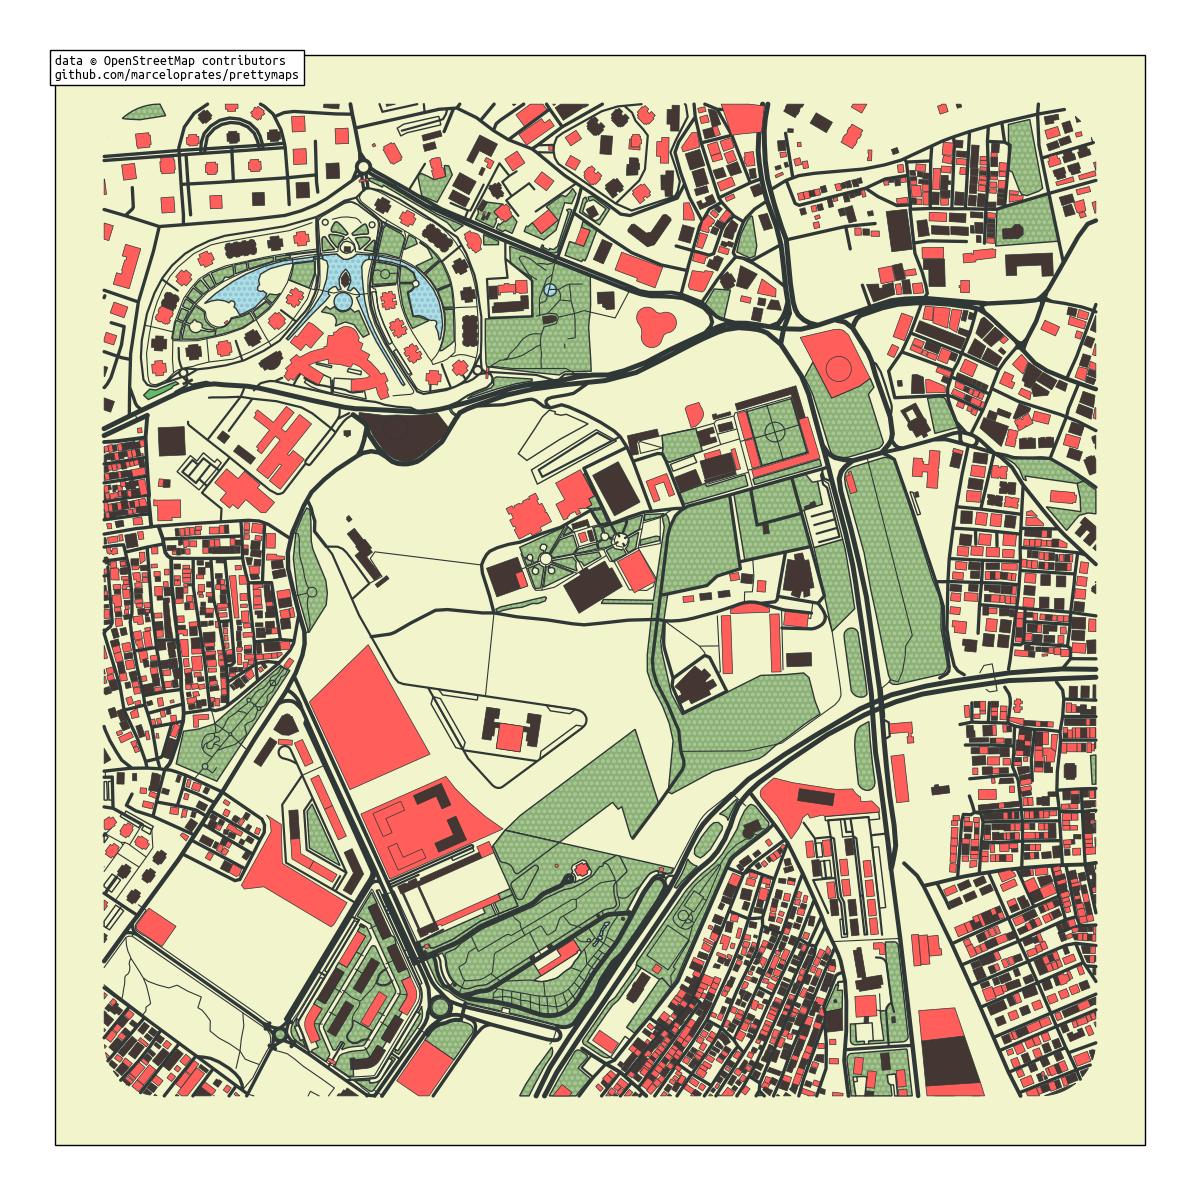
\includegraphics[width=0.5\textwidth]{images/izu.png}
    \caption{Prettymaps IZU.}
    \label{fig:enter-label}
\end{figure}

\newpage

\subsection{Scikeras - Keras HP Tuning}
\begin{lstlisting}[language=Python]
import tensorflow as tf
from scikeras.wrappers import KerasClassifier
from sklearn.model_selection import GridSearchCV

def create_model(units=16, lr_rate=0.1):
    model = tf.keras.Sequential()
    model.add(tf.keras.layers.Dense(units, activation='relu'))
    model.add(tf.keras.layers.Dense(num_classes, activation='softmax'))
    model.compile(optimizer=tf.keras.optimizers.Adam(learning_rate=lr_rate),
                  loss='categorical_crossentropy',
                  metrics=['accuracy'])
    return model

units = [16, 32]
lr_rate = [0.1,0.001]
batch_size = [128, 64]

keras_model = KerasClassifier(build_fn=create_model, 
                              units=units, 
                              lr_rate=lr_rate, 
                              epochs=10, 
                              batch_size=batch_size, 
                              callbacks=[EarlyStopping(monitor='val_loss', patience=3)], 
                              verbose=0)

param_grid = dict(units = units, lr_rate = lr_rate, batch_size = batch_size)
grid = GridSearchCV(estimator = keras_model, param_grid = param_grid, cv = 3)
grid_result = grid.fit(train_data, train_labels)
print("The best parameters are:",grid_result.best_params_)
best_params = grid_result.best_params_
\end{lstlisting}

\subsection{pyLDAvis - Topic Modeling with LDA}
\begin{lstlisting}[language=Python]
import gensim
import pyLDAvis.gensim

tokenized = df["Lemmatization"]
tokenized = [token.split(" ") for token in tokenized]
dictionary = corpora.Dictionary(tokenized)
dictionary.filter_extremes(no_below=1, no_above=0.8)
corpus = [dictionary.doc2bow(tokens) for tokens in tokenized]

ldamodel = gensim.models.ldamodel.LdaModel(corpus, num_topics = 8, id2word=dictionary, passes=15)
lda_display = pyLDAvis.gensim.prepare(ldamodel, corpus, dictionary, sort_topics=True)
pyLDAvis.display(lda_display)
\end{lstlisting}

\subsection{visualkeras - 3D Model Visualization}
\begin{lstlisting}[language=Python]
import tensorflow as tf
import visualkeras

model = tf.keras.Sequential()
model.add(tf.keras.layers.Conv2D(32, (3, 3), activation='relu', input_shape=(224, 224, 3)))
model.add(tf.keras.layers.MaxPooling2D((2, 2)))
model.add(tf.keras.layers.Conv2D(64, (3, 3), activation='relu'))
model.add(tf.keras.layers.MaxPooling2D((2, 2)))
model.add(tf.keras.layers.Conv2D(64, (3, 3), activation='relu'))
model.add(tf.keras.layers.Flatten())
model.add(tf.keras.layers.Dense(32, activation='relu'))
model.add(tf.keras.layers.Dense(10, activation='softmax'))
model.compile(optimizer=tf.keras.optimizers.Adam(),
              loss='categorical_crossentropy',
              metrics=['accuracy'])

visualkeras.layered_view(model, to_file="visualkeras.png").show()
\end{lstlisting}

\begin{figure}[ht]
    \centering
    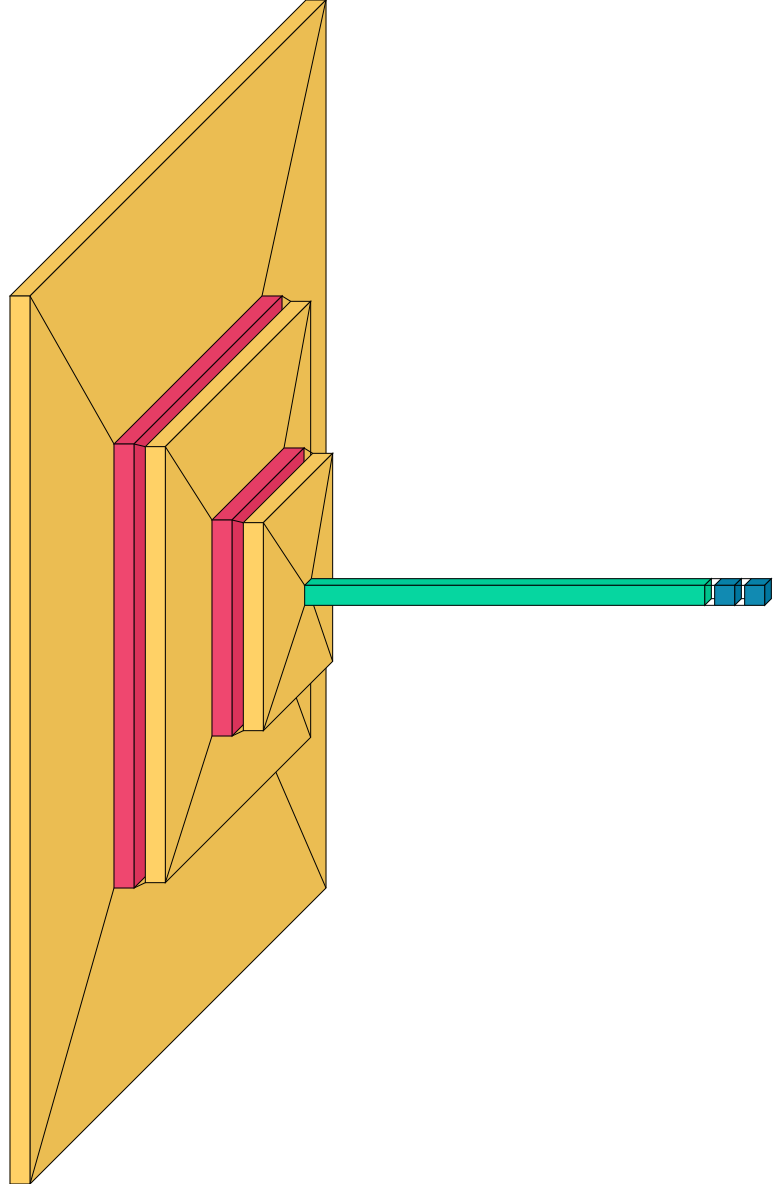
\includegraphics[width=0.25\textwidth]{images/visualkeras.png}
    \caption{visualkeras .}
    \label{fig:enter-label}
\end{figure}

\newpage

\subsection{Plotting N-Grams}
\begin{lstlisting}[language=Python]
def count_ngrams(corpus, ngram, n):
    vec = CountVectorizer(ngram_range=(ngram,ngram)).fit(corpus)
    bag_of_words = vec.transform(corpus)
    sum_words = bag_of_words.sum(axis=0)
    words_freq = [(word, sum_words[0, idx]) for word, idx in vec.vocabulary_.items()]
    words_freq =sorted(words_freq, key = lambda x: x[1], reverse=True)
    return words_freq[:n]
    
def plot_ngrams(ngram_df, ngram_name):
    plt.figure(figsize=(12, 6))
    plt.bar(data=ngram_df, x="Tweets", height="Count")
    plt.xticks(rotation=90)
    plt.xlabel(ngram_name)
    plt.ylabel("Count")
    plt.title(ngram_name)
    plt.show()
    
unigrams = count_ngrams(corpus=df["Lemmatization"], ngram=1, n=30)
top_unigram = pd.DataFrame(unigrams, columns=['Tweets', "Count"])
plot_ngrams(top_unigram, "Unigrams")
\end{lstlisting}

\begin{figure}[ht]
    \centering
    \includegraphics[width=1.0\textwidth]{images/nlp_unigram.png}
    \caption{Unigrams .}
    \label{fig:enter-label}
\end{figure}

\newpage

\subsection{Matplotlib Styles}
\subsubsection{XKCD Style}
\begin{lstlisting}[language=Python]
import matplotlib.pyplot as plt
import pandas as pd

df = pd.DataFrame({
    'x': [1, 2, 2.5, 3, 3.5, 4, 5],
    'y': [5, 10, 12.5, 15, 17.5, 20, 25],
})
 
with plt.xkcd():
    plt.rcParams['figure.figsize'] = [12, 8]
    fig1 = plt.figure()
    ax = df.plot.bar()

plt.show()
\end{lstlisting}

\begin{figure}[ht]
    \centering
    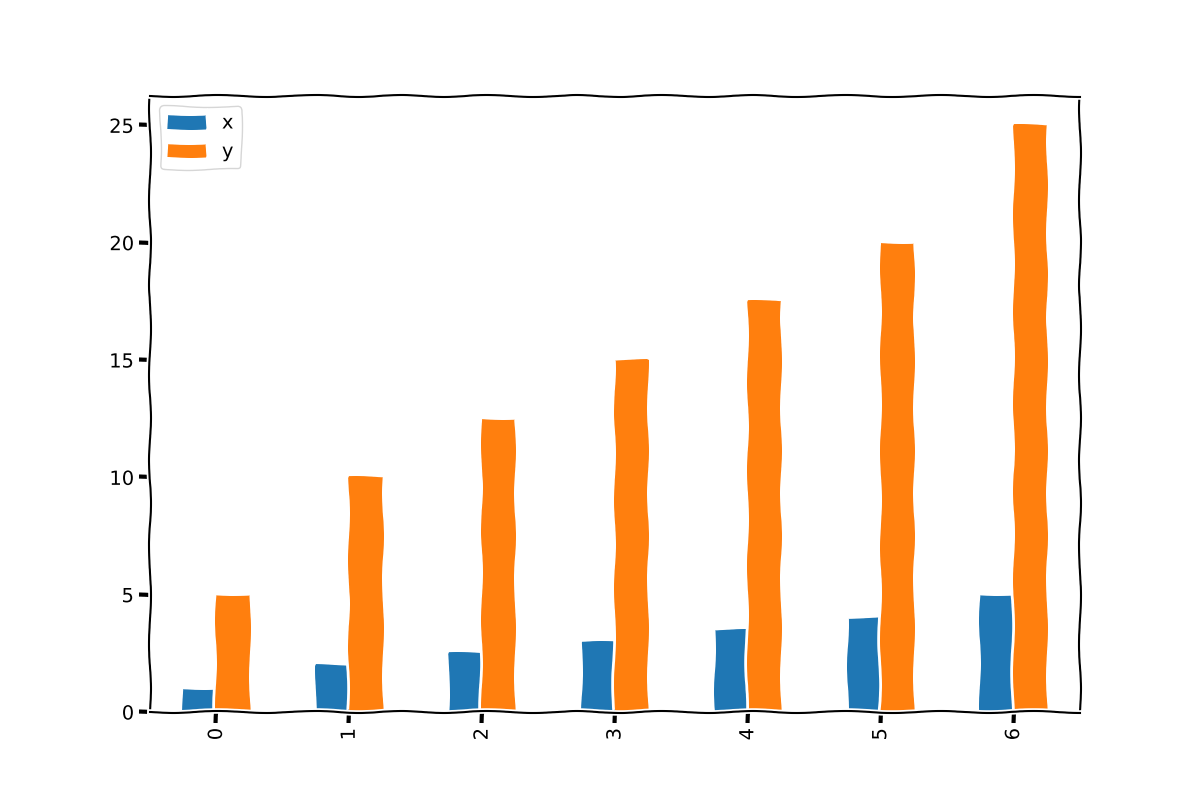
\includegraphics[width=1.0\textwidth]{images/style_xkcd.png}
    \caption{XKCD Style .}
    \label{fig:enter-label}
\end{figure}

\newpage

\subsection{Scikit-Learn-Intelex: Intel sistemlerde Sklearn hızlandırma}
\subsubsection{Intel CPU'lar için}
\begin{lstlisting}[language=Python]
from sklearnex import patch_sklearn
patch_sklearn()

from sklearn.cluster import DBSCAN
\end{lstlisting}

\subsubsection{Intel GPU'lar için}
\begin{lstlisting}[language=Python]
import dpctl
from sklearnex import patch_sklearn, config_context
patch_sklearn()

from sklearn.cluster import DBSCAN

with config_context(target_offload='gpu:0'):
	model = DBSCAN()
\end{lstlisting}

\subsection{Deepchecks - Model Validation}
\subsubsection{Model Evaluation}
\begin{lstlisting}[language=Python]
import pandas as pd
import numpy as np
from sklearn import datasets
from sklearn.model_selection import train_test_split
from sklearn.ensemble import RandomForestClassifier

from deepchecks.tabular import Dataset
from deepchecks.suites import model_evaluation

df  = datasets.load_breast_cancer(as_frame=True).frame
label = 'target'
train_df, test_df = train_test_split(df, test_size=0.2, random_state=123)

train = Dataset(train_df, label=label)
test = Dataset(test_df, label=label)

x_train = train_df.drop(label, axis = 1)
y_train = train_df[label]
x_test = test_df.drop(label, axis = 1)
y_test = test_df[label]

model = RandomForestClassifier()
model.fit(x_train, y_train)

suite = model_evaluation()
suite_result = suite.run(train_dataset=train, test_dataset=test, model=model)
suite_result.save_as_html()
\end{lstlisting}

\subsubsection{Data Consistency Check}
\begin{lstlisting}[language=Python]
from deepchecks.suites import  train_test_validation

data_consistency_check = train_test_validation()
data_consistency_check.run(model=model, train_dataset=train, test_dataset=test)
\end{lstlisting}

\subsubsection{Data Purity Check}
\begin{lstlisting}[language=Python]
from deepchecks.suites import data_integrity

purity_check = data_integrity()
purity_check.run(train_dataset = train)
\end{lstlisting}

\subsection{Pandas Profiling}
\begin{lstlisting}[language=Python]
from pandas_profiling import ProfileReport

profile = ProfileReport(
    df, title="", html={"style": {"full_width": True}}, sort=None
)
profile
\end{lstlisting}

\newpage

\subsection{PDPBOX - Partial Dependence Plot}
\begin{lstlisting}[language=Python]
from pdpbox import pdp, get_example, info_plots

target_radius = info_plots.TargetPlot(
    df=df,
    feature="mean radius",
    feature_name="mean radius",
    target='target',
)
fig, axes, summary_df = target_radius.plot(
    figsize=None,
    ncols=2,
    plot_params=None,
    engine='plotly',
    template='plotly_white',
)
fig.update_layout()
\end{lstlisting}

\begin{figure}[ht]
    \centering
    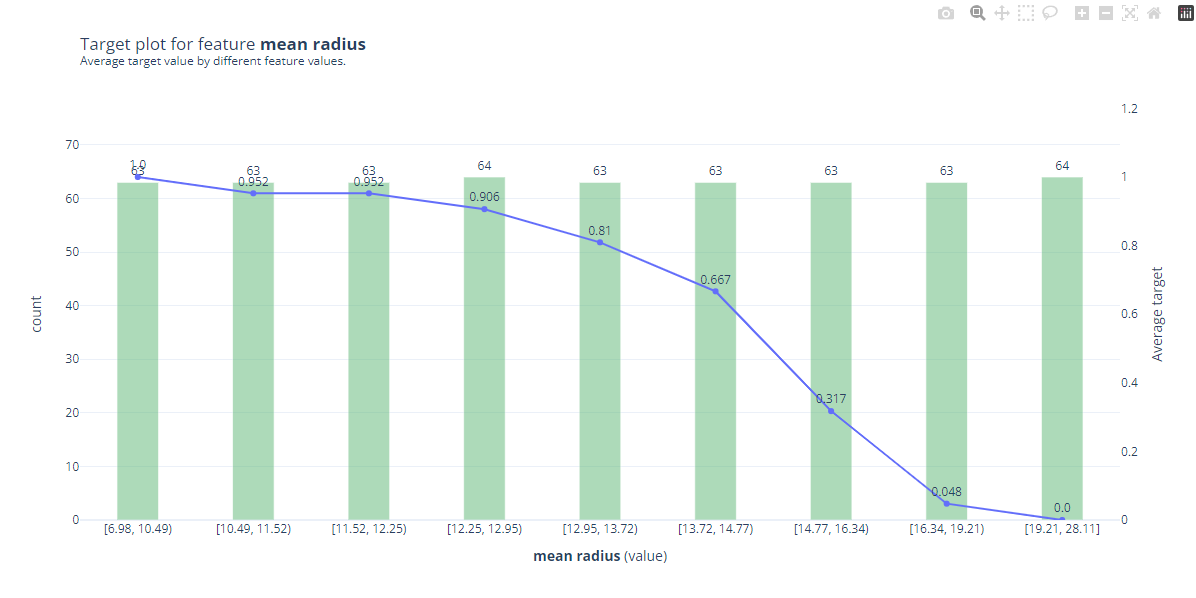
\includegraphics[width=1.0\textwidth]{images/pdpbox_demo.png}
    \caption{pdpbox demo}
    \label{fig:enter-label}
\end{figure}

\newpage

\subsection{dtreeviz  vs plot\_tree - Tree Visualization}
\subsubsection{dtreeviz}
\begin{lstlisting}[language=Python]
import dtreeviz

viz = dtreeviz.model(
    model,
    x_train,
    y_train,
    target_name="target",
    feature_names=list(x_train.columns)
)
viz.view(scale=1.3)
\end{lstlisting}

\begin{figure}[ht]
    \centering
    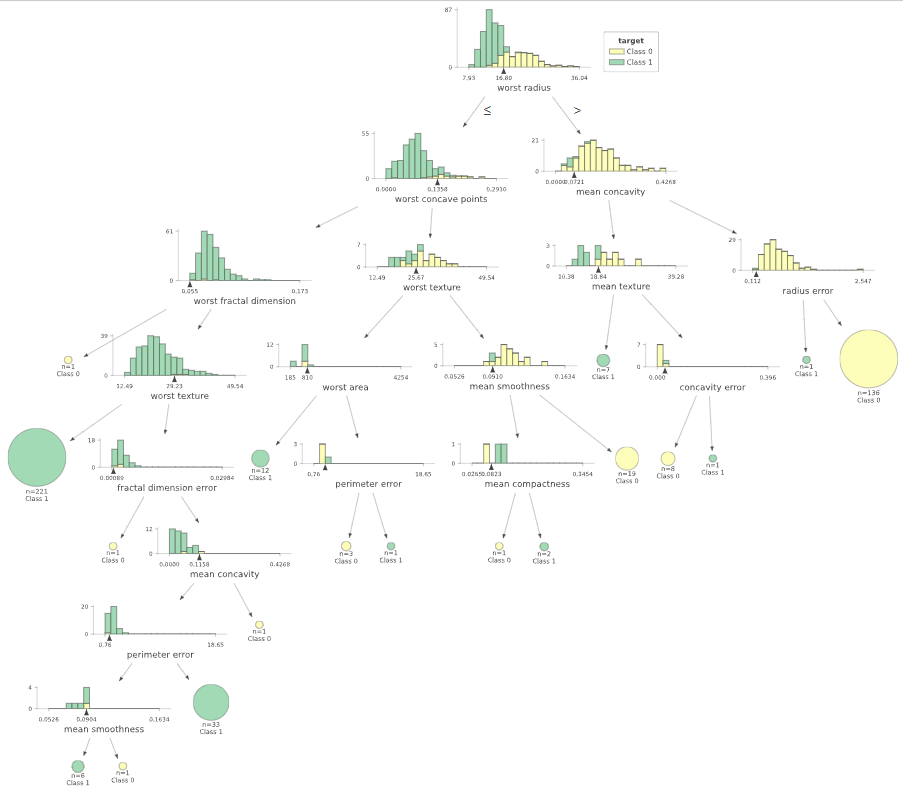
\includegraphics[width=1.0\textwidth]{images/dtreeviz.png}
    \caption{pdpbox demo}
    \label{fig:enter-label}
\end{figure}

\newpage

\subsubsection{tree.plot\_tree}
\begin{lstlisting}[language=Python]
from sklearn.tree import plot_tree

fig, axes = plt.subplots(figsize=(25,22))
plot_tree(model, filled = True)
plt.savefig("plot_tree.png")
plt.show()
\end{lstlisting}

\begin{figure}[ht]
    \centering
    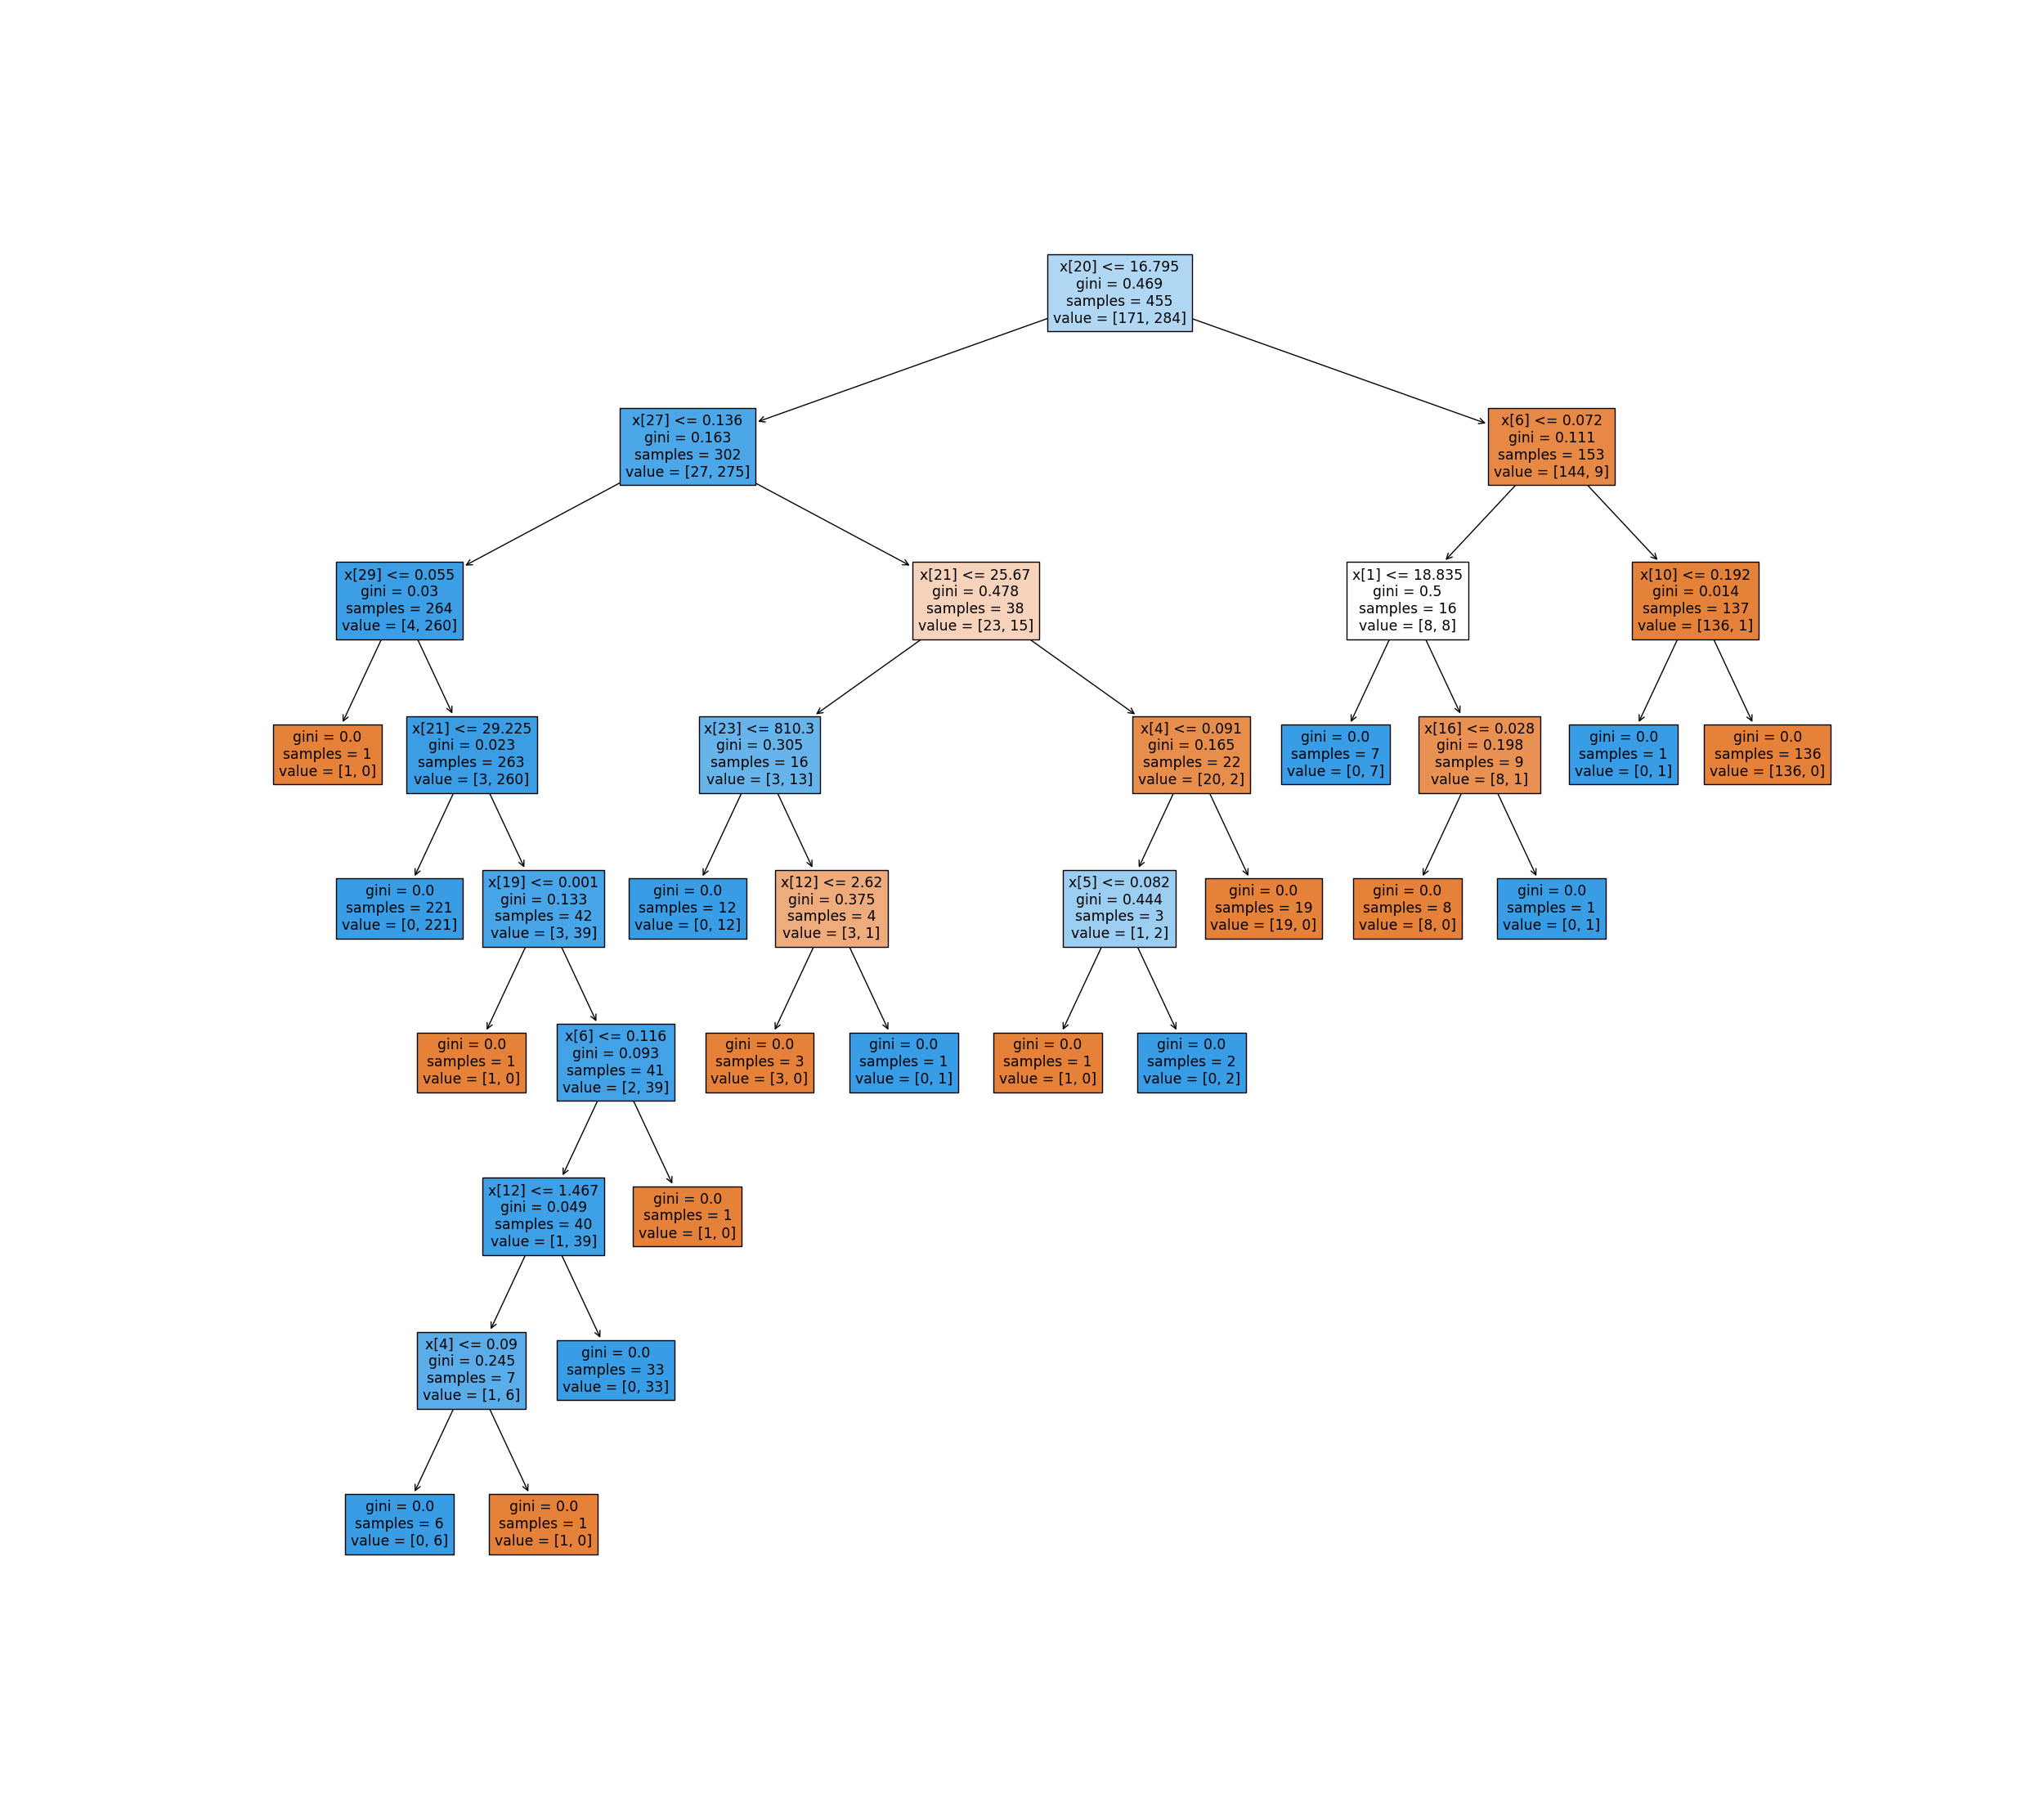
\includegraphics[width=1.0\textwidth]{images/plot_tree.png}
    \caption{pdpbox demo}
    \label{fig:enter-label}
\end{figure}

\newpage

\subsection{SKompiler - Model Algoritması Dönüşümü}
\begin{lstlisting}[language=Python]
import numpy as np
from sklearn.datasets import load_iris
from sklearn.tree import DecisionTreeClassifier
from skompiler import skompile

iris = load_iris()
model = DecisionTreeClassifier(max_depth=3)
model.fit(iris.data, iris.target)
js_code = skompile(model.predict).to('sympy/js')
# if (x[2] <= 2.44999998807907) {
#    y = 0;
# }
# else {
#    if (x[3] <= 1.75) {
#       if (x[2] <= 4.95000004768372) {
#          y = 1;
#       }
#       else {
#          y = 2;
#       }
#    }
#    else {
#       y = 2;
#    }
# }
\end{lstlisting}

\subsection{dtype\_diet - Veri Tipi Optimizasyonu}
dtype\_diet veri tipi optimizasyonu yaparak veri tiplerinin bellek kullanımını azaltmayı hedefler.

\begin{lstlisting}[language=Python]
import pandas as pd
from dtype_diet import report_on_dataframe, optimize_dtypes

df = pd.read_csv("/mnt/d/Datasets/kddcup/kddcup.data.corrected")
m1 = df.memory_usage(deep=True).sum() / 1024 / 1024
print(f"Original df memory: {m1} MB")
# Original df memory: 2567.740376472473 MB

proposed_df = report_on_dataframe(df, unit="MB")
new_df = optimize_dtypes(df, proposed_df)
m2 = new_df.memory_usage(deep=True).sum() / 1024 / 1024
print(f"Optimized df memory: {m2} MB")
# Optimized df memory: 756.7935743331909 MB
\end{lstlisting}

\newpage

\subsection{SWMat - Grafik İşlemleri}
\begin{lstlisting}[language=Python]
import matplotlib.pyplot as plt
from SWMat.SWMat import SWMat

data = [1, 1, 2, 3, 5, 1, 2, 
        4, 4, 4, 3, 5, 6, 3, 
        5, 5, 3, 3, 1, 2, 3, 
        4, 5, 6, 6, 5, 4, 3, 4, 5]
swm = SWMat(plt) 
swm.violinplot(data, highlight={"0":[(0.5, 2.5), (4.5, 6)]});
swm.text("Some text");
plt.savefig("swmat.png")
\end{lstlisting}

\begin{figure}[ht]
    \centering
    
\includegraphics[width=1.0\textwidth]{images/swmat.png}
    \caption{swmat demo}
    \label{fig:enter-label}
\end{figure}

\newpage

\subsection{scattertext - NLP Scatter Text Graph}
\begin{lstlisting}[language=Python]
import pandas as pd
import scattertext as st

df = pd.read_csv("/mnt/d/Datasets/data.csv")
df = df.assign(
    parse=lambda df: df.text.apply(st.whitespace_nlp_with_sentences)
)
corpus = st.CorpusFromParsedDocuments(
    df, 
    category_col='category', 
    parsed_col='parse'
).build().get_unigram_corpus().compact(st.AssociationCompactor(2000))
html = st.produce_scattertext_explorer(
    corpus,
    category='siyaset ',
    category_name='Siyaset',
    not_category_name='Dunya',
    minimum_term_frequency=0, 
    pmi_threshold_coefficient=0,
    width_in_pixels=1000, 
    metadata=corpus.get_df()['category'],
    transform=st.Scalers.dense_rank,
)
open('./scattertext.html', 'w').write(html)
\end{lstlisting}

\begin{figure}[ht]
    \centering
    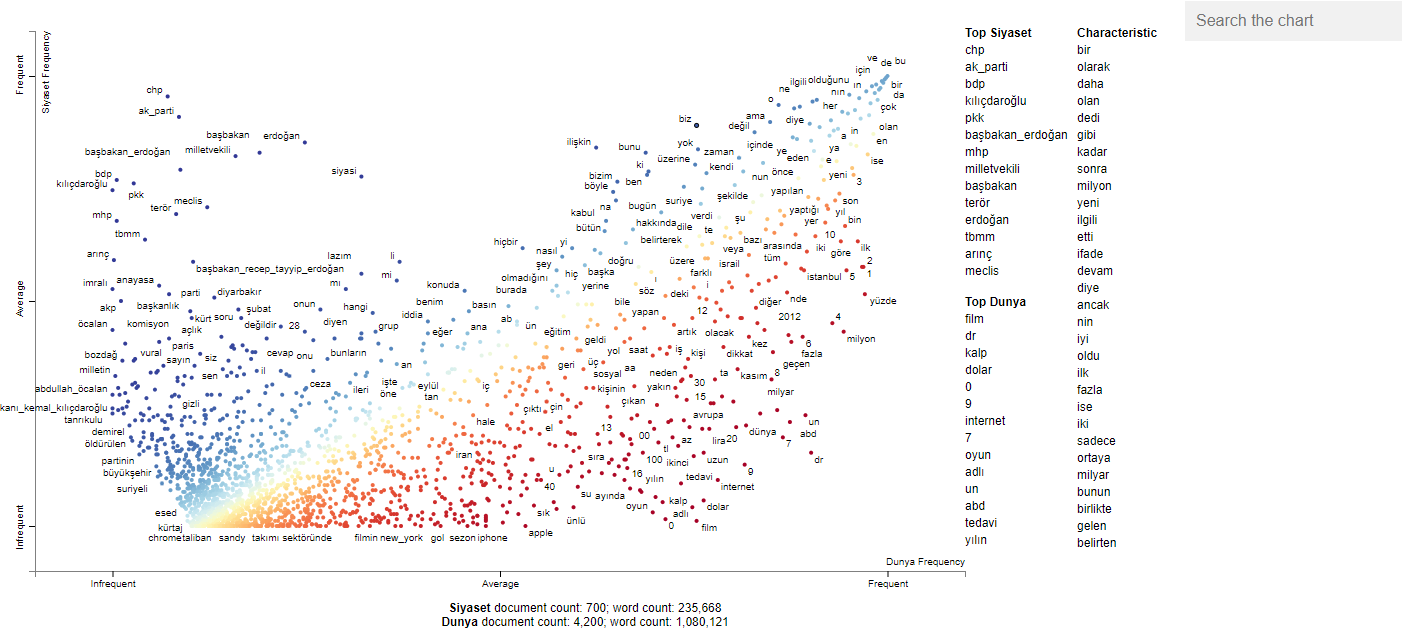
\includegraphics[width=1.0\textwidth]{images/scattertext.png}
    \caption{scattertext demo}
    \label{fig:enter-label}
\end{figure}

\newpage

\subsection{albumentations - Image Augmentation}
\begin{lstlisting}[language=Python]
import os
import cv2
import numpy as np
from albumentations import Compose, HorizontalFlip, RandomBrightnessContrast, Rotate
from albumentations.augmentations.transforms import Resize

input_dir = ''
output_dir = ''

augmentation_pipeline = Compose([
    HorizontalFlip(p=0.5),
    RandomBrightnessContrast(p=0.5),
    Rotate(limit=45, p=0.5),
    Resize(height=256, width=256, p=1)
])

for filename in os.listdir(input_dir):
    if filename.endswith(".jpg") or filename.endswith(".png"):
        image_path = os.path.join(input_dir, filename)
        image = cv2.imread(image_path)
        if image is None:
            continue

        augmented = augmentation_pipeline(image=image)
        augmented_image = augmented['image']

        base_filename, ext = os.path.splitext(filename)
        new_filename = f"{base_filename}_augmented{ext}"
        output_path = os.path.join(output_dir, new_filename)
        cv2.imwrite(output_path, augmented_image)
\end{lstlisting}

\newpage